\chapter{Software Requirement Specification}

%%%%%%%%%%%%%%%%%%%%%%%%%%%%%%%%%%%%%%%%%%%%%%%%%%%%%%%%%%%%%%%%%%%%%%
\section{Product Overview}

% Phần này do thành viên khác thực hiện.

%%%%%%%%%%%%%%%%%%%%%%%%%%%%%%%%%%%%%%%%%%%%%%%%%%%%%%%%%%%%%%%%%%%%%%
\section{User Requirements}


%%%%%%%%%%%%%%%%%%%%%%%%%%%%%%%%%%%%%%%%%%%%%%%%%%%%%%%%%%%%%%%%%%%%%%
\section{Functional Requirements}


\subsection{System Functional Overview}


%%%%%%%%%%%%%%%%%%%%%%%%%%%%%%%%%%%%%%%%%%%%%%%%%%%%%%%%%%%%%%%%%%%%%%
\subsection{Authentication}

Authentication is responsible for verifying user identities before allowing access to the Personalized Career Orientation \& Learning Roadmap Platform. This module provides secure login, user registration, password recovery, and logout functions. Only authenticated users can access system resources according to their assigned roles.

%%%%%%%%%%%%%%%%%%%%%%%%%%%%%%%%%%%%%%%%%%%%%%%%%%%%%%%%%%%%%%%%%%%%%%
\subsubsection{Login}

\textbf{Role:}

Student, Mentor, Career Counselor, Administrator.

\vspace{0.3cm}

\textbf{Function Trigger:}

The user enters a registered email address and password, then clicks the \textbf{Login} button.

\vspace{0.3cm}

\textbf{Function Description:}

\begin{itemize}
    \item \textbf{Purpose:}

    Authenticate users before granting access to the system.

    \item \textbf{Data Processing:}

    The system validates the entered credentials, verifies the account status, authenticates the user, determines the user role, and redirects the user to the corresponding dashboard.
\end{itemize}

\vspace{0.3cm}

\textbf{Function Details:}

\begin{itemize}
    \item If the login credentials are correct, the system redirects the user to the corresponding dashboard.

    \item If the email address or password is incorrect, the system displays an error message.

    \item If the account has not been verified, the system requests email verification before login.

    \item If the account is temporarily locked because of multiple unsuccessful login attempts, the system informs the user accordingly.
\end{itemize}

%%%%%%%%%%%%%%%%%%%%%%%%%%%%%%%%%%%%%%%%%%%%%%%%%%%%%%%%%%%%%%%%%%%%%%
%\begin{figure}[H]
%    \centering
%    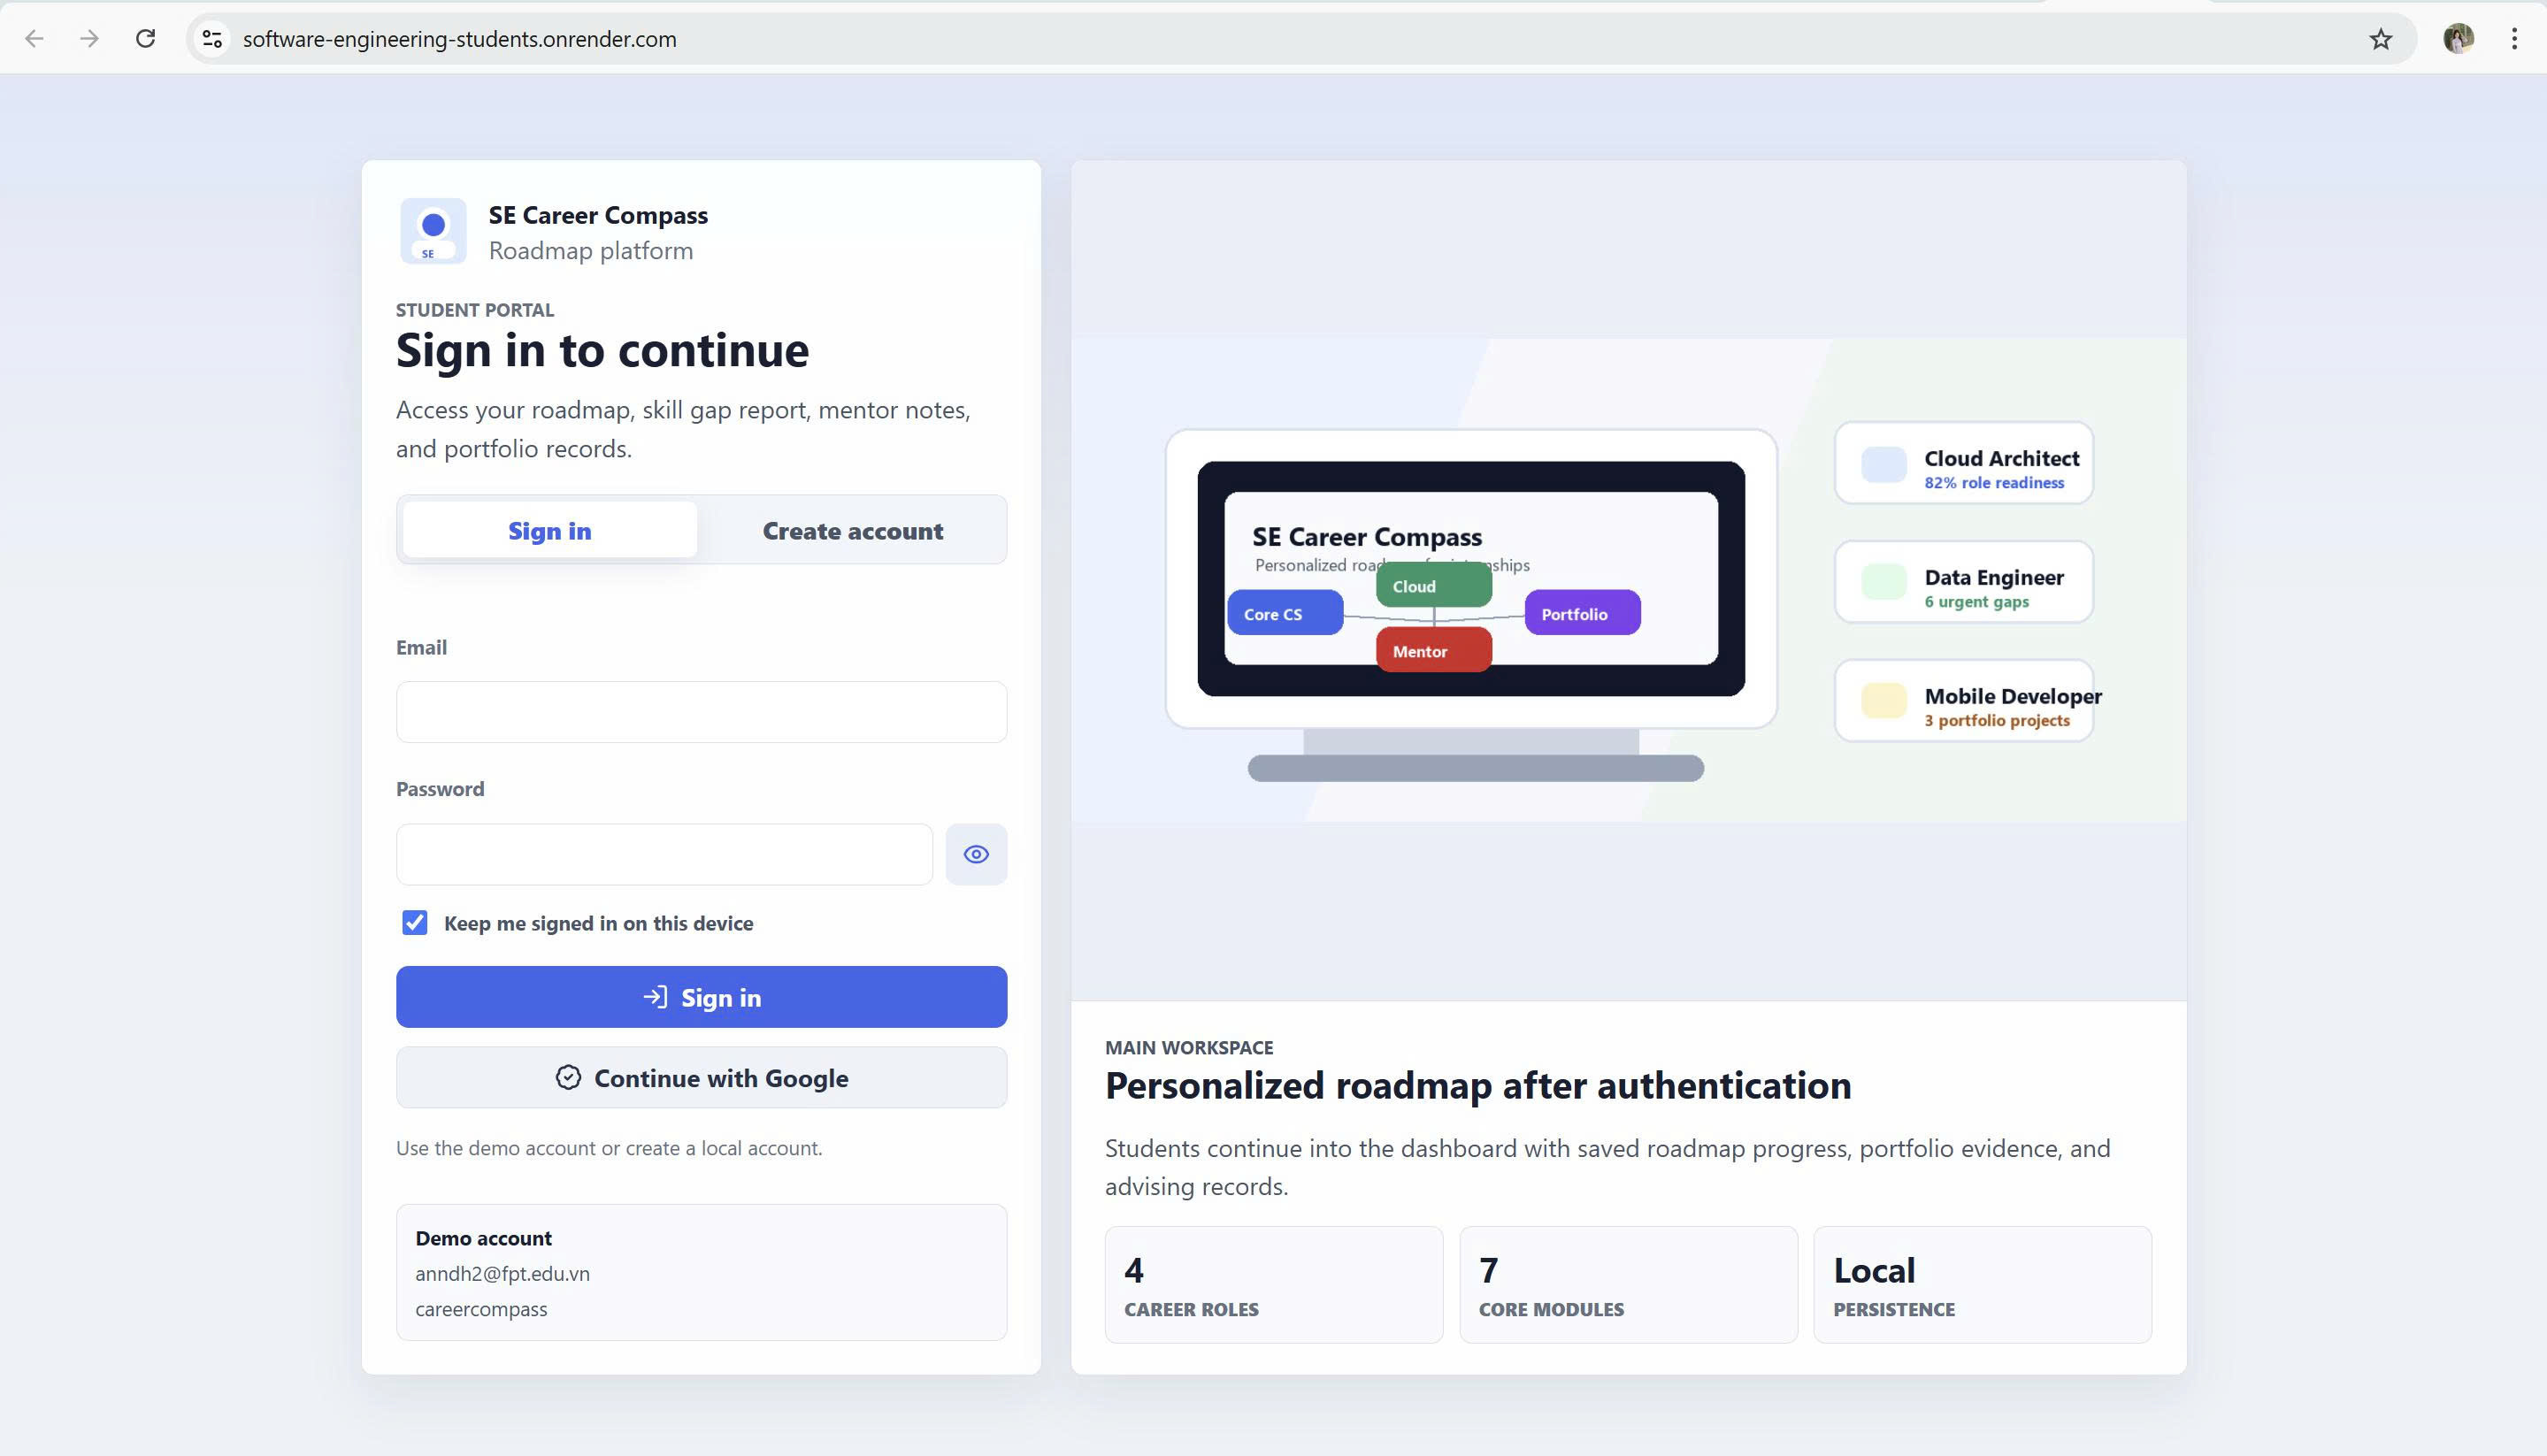
\includegraphics[width=0.9\textwidth]{images/login.png}
%    \caption{Login Interface}
%    \label{fig:login_interface}
%\end{figure}


%%%%%%%%%%%%%%%%%%%%%%%%%%%%%%%%%%%%%%%%%%%%%%%%%%%%%%%%%%%%%%%%%%%%%%
\subsection{User Management}

User Management is responsible for managing user accounts and personal information within the Personalized Career Orientation \& Learning Roadmap Platform. This module enables administrators to maintain user accounts, while users can update their own profile information. The system also supports searching, viewing, editing, and deleting user accounts according to role-based access permissions.
%%%%%%%%%%%%%%%%%%%%%%%%%%%%%%%%%%%%%%%%%%%%%%%%%%%%%%%%%%%%%%%%%%%%%%
\subsubsection{Manage Users}

\textbf{Role:}

Administrator.

\vspace{0.3cm}

\textbf{Function Trigger:}

The administrator logs into the system and navigates to the \textbf{User Management} page.

\vspace{0.3cm}

\textbf{Function Description:}

\begin{itemize}
    \item \textbf{Purpose:}

    Manage all user accounts in the system.

    \item \textbf{Data Processing:}

    Create, edit, delete, search, and update user account information.
\end{itemize}

\vspace{0.3cm}

\textbf{Function Details:}

\begin{itemize}
    \item The administrator can create new user accounts.

    \item The administrator can update user information.

    \item The administrator can activate or deactivate user accounts.

    \item Search users by Student ID, Full Name, or Email Address.

    \item Assign roles such as Student, Mentor, Career Counselor, or Administrator.
\end{itemize}

%%%%%%%%%%%%%%%%%%%%%%%%%%%%%%%%%%%%%%%%%%%%%%%%%%%%%%%%%%%%%%%%%%%%%%
% Figure 1: User List
%
% \begin{figure}[H]
%     \centering
%     \includegraphics[width=0.95\textwidth]{images/manage_users_list.png}
%     \caption{User Management Interface}
%     \label{fig:manage_users_list}
% \end{figure}
%%%%%%%%%%%%%%%%%%%%%%%%%%%%%%%%%%%%%%%%%%%%%%%%%%%%%%%%%%%%%%%%%%%%%%

%%%%%%%%%%%%%%%%%%%%%%%%%%%%%%%%%%%%%%%%%%%%%%%%%%%%%%%%%%%%%%%%%%%%%%
% Figure 2: Create User
%
% \begin{figure}[H]
%     \centering
%     \includegraphics[width=0.95\textwidth]{images/create_user.png}
%     \caption{Create User Interface}
%     \label{fig:create_user}
% \end{figure}
%%%%%%%%%%%%%%%%%%%%%%%%%%%%%%%%%%%%%%%%%%%%%%%%%%%%%%%%%%%%%%%%%%%%%%

%%%%%%%%%%%%%%%%%%%%%%%%%%%%%%%%%%%%%%%%%%%%%%%%%%%%%%%%%%%%%%%%%%%%%%
% Figure 3: Edit User
%
% \begin{figure}[H]
%     \centering
%     \includegraphics[width=0.95\textwidth]{images/edit_user.png}
%     \caption{Edit User Interface}
%     \label{fig:edit_user}
% \end{figure}
%%%%%%%%%%%%%%%%%%%%%%%%%%%%%%%%%%%%%%%%%%%%%%%%%%%%%%%%%%%%%%%%%%%%%%

%%%%%%%%%%%%%%%%%%%%%%%%%%%%%%%%%%%%%%%%%%%%%%%%%%%%%%%%%%%%%%%%%%%%%%
\subsubsection{Import Students}

\textbf{Role:}

Administrator.

\vspace{0.3cm}

\textbf{Function Trigger:}

The administrator logs into the system, opens the \textbf{User Management} module, and selects the \textbf{Import Students} function.

\vspace{0.3cm}

\textbf{Function Description:}

\begin{itemize}
    \item \textbf{Purpose:}

    Import student accounts into the system.

    \item \textbf{Data Processing:}

    Read student information from an Excel file and automatically create user accounts.
\end{itemize}

\vspace{0.3cm}

\textbf{Function Details:}

\begin{itemize}
    \item Import student information from an Excel file.

    \item Validate duplicated Student IDs and email addresses.

    \item Automatically assign the Student role.

    \item Display the import result after processing.
\end{itemize}

%%%%%%%%%%%%%%%%%%%%%%%%%%%%%%%%%%%%%%%%%%%%%%%%%%%%%%%%%%%%%%%%%%%%%%
% \begin{figure}[H]
%     \centering
%     \includegraphics[width=0.9\textwidth]{images/import_students.png}
%     \caption{Import Students Interface}
%     \label{fig:import_students}
% \end{figure}

%%%%%%%%%%%%%%%%%%%%%%%%%%%%%%%%%%%%%%%%%%%%%%%%%%%%%%%%%%%%%%%%%%%%%%
\subsubsection{Import Mentors}

\textbf{Role:}

Administrator.

\vspace{0.3cm}

\textbf{Function Trigger:}

The administrator logs into the system, opens the \textbf{User Management} module, and selects the \textbf{Import Mentors} function.

\vspace{0.3cm}

\textbf{Function Description:}

\begin{itemize}
    \item \textbf{Purpose:}

    Import mentor accounts into the system.

    \item \textbf{Data Processing:}

    Read mentor information from an Excel file and create mentor accounts automatically.
\end{itemize}

\vspace{0.3cm}

\textbf{Function Details:}

\begin{itemize}
    \item Import mentor information from an Excel file.

    \item Validate duplicated email addresses.

    \item Automatically assign the Mentor role.

    \item Display the import result after processing.
\end{itemize}

%%%%%%%%%%%%%%%%%%%%%%%%%%%%%%%%%%%%%%%%%%%%%%%%%%%%%%%%%%%%%%%%%%%%%%
% \begin{figure}[H]
%     \centering
%     \includegraphics[width=0.9\textwidth]{images/import_mentors.png}
%     \caption{Import Mentors Interface}
%     \label{fig:import_mentors}
% \end{figure}

%%%%%%%%%%%%%%%%%%%%%%%%%%%%%%%%%%%%%%%%%%%%%%%%%%%%%%%%%%%%%%%%%%%%%%
\subsection{Career Assessment Management}

Career Assessment Management allows students to evaluate their technical skills, interests, and career orientation through assessment questionnaires. The assessment results are analyzed by the system and used as the basis for generating personalized career recommendations and learning roadmaps.
%%%%%%%%%%%%%%%%%%%%%%%%%%%%%%%%%%%%%%%%%%%%%%%%%%%%%%%%%%%%%%%%%%%%%%
\subsubsection{Student Take Career Assessment}

\textbf{Function Trigger:}

Student logs in $\rightarrow$ navigates to \textbf{"Career Assessment"} $\rightarrow$ clicks \textbf{"Start Assessment"}.

\vspace{0.3cm}

\textbf{Function Description:}

\textbf{Actors:}

Student

\vspace{0.2cm}

\textbf{Purpose:}

Allow students to evaluate their technical skills, interests, and career orientation.

\vspace{0.2cm}

\textbf{Interface:}

An assessment page containing multiple-choice questions related to programming, software engineering knowledge, career interests, and technical skills.

\vspace{0.2cm}

\textbf{Data Processing:}

The student's answers are saved in the database. The system calculates the assessment score and generates an assessment result for future AI recommendations.

\vspace{0.3cm}

\textbf{Function Details:}

\textbf{Validation:}

\begin{itemize}
\item All questions must be answered.
\end{itemize}

\textbf{Business Rules:}

\begin{itemize}
\item Students can take the assessment once per evaluation period.
\item Assessment results are stored for future comparison.
\end{itemize}

\textbf{Normal Case:}

Student answers all questions $\rightarrow$ clicks \textbf{"Submit"} $\rightarrow$ system calculates the score and saves the result.

\textbf{Abnormal Case:}

If required questions are unanswered, the system requests the student to complete all questions before submission.

%%%%%%%%%%%%%%%%%%%%%%%%%%%%%%%%%%%%%%%%%%%%%%%%%%%%%%%%%%%%%%%%%%%%%%
% Figure 1: Career Assessment Interface
%
% \begin{figure}[H]
%     \centering
%     \includegraphics[width=0.95\textwidth]{images/career_assessment.png}
%     \caption{Career Assessment Interface}
%     \label{fig:career_assessment}
% \end{figure}
%%%%%%%%%%%%%%%%%%%%%%%%%%%%%%%%%%%%%%%%%%%%%%%%%%%%%%%%%%%%%%%%%%%%%%

%%%%%%%%%%%%%%%%%%%%%%%%%%%%%%%%%%%%%%%%%%%%%%%%%%%%%%%%%%%%%%%%%%%%%%
\subsubsection{View Assessment Result}

\textbf{Function Trigger:}

Student completes the assessment $\rightarrow$ selects \textbf{"View Result"}.

\vspace{0.3cm}

\textbf{Function Description:}

\textbf{Actors:}

Student

\vspace{0.2cm}

\textbf{Purpose:}

Allow students to review their assessment results.

\vspace{0.2cm}

\textbf{Interface:}

A result page displaying assessment score, strengths, weaknesses, and suggested career paths.

\vspace{0.2cm}

\textbf{Data Processing:}

Retrieve assessment results from the database and display them graphically.

\vspace{0.3cm}

\textbf{Function Details:}

\textbf{Business Rules:}

\begin{itemize}
\item Students can only view their own assessment results.
\end{itemize}

\textbf{Normal Case:}

Student selects \textbf{"View Result"} $\rightarrow$ system displays assessment report.

\textbf{Abnormal Case:}

If no assessment exists, the system requests the student to complete an assessment first.

%%%%%%%%%%%%%%%%%%%%%%%%%%%%%%%%%%%%%%%%%%%%%%%%%%%%%%%%%%%%%%%%%%%%%%
% Figure 2: Assessment Result Interface
%
% \begin{figure}[H]
%     \centering
%     \includegraphics[width=0.95\textwidth]{images/assessment_result.png}
%     \caption{Assessment Result Interface}
%     \label{fig:assessment_result}
% \end{figure}
%%%%%%%%%%%%%%%%%%%%%%%%%%%%%%%%%%%%%%%%%%%%%%%%%%%%%%%%%%%%%%%%%%%%%%

%%%%%%%%%%%%%%%%%%%%%%%%%%%%%%%%%%%%%%%%%%%%%%%%%%%%%%%%%%%%%%%%%%%%%%
\subsubsection{Mentor Review Assessment}

\textbf{Function Trigger:}

Mentor logs in $\rightarrow$ navigates to \textbf{"Student Assessments"} $\rightarrow$ selects a student.

\vspace{0.3cm}

\textbf{Function Description:}

\textbf{Actors:}

Mentor

\vspace{0.2cm}

\textbf{Purpose:}

Review students' assessment results and provide career guidance.

\vspace{0.2cm}

\textbf{Interface:}

A dashboard displaying assessment reports, skill analysis, and feedback form.

\vspace{0.2cm}

\textbf{Data Processing:}

Store mentor comments and recommendations in the database.

\vspace{0.3cm}

\textbf{Function Details:}

\textbf{Business Rules:}

\begin{itemize}
\item Mentors can only review students assigned to them.
\end{itemize}

\textbf{Normal Case:}

Mentor reviews assessment $\rightarrow$ enters comments $\rightarrow$ clicks \textbf{"Save Feedback"}.

\textbf{Abnormal Case:}

If the selected student has not completed an assessment, the system displays a notification.

%%%%%%%%%%%%%%%%%%%%%%%%%%%%%%%%%%%%%%%%%%%%%%%%%%%%%%%%%%%%%%%%%%%%%%
% Figure 3: Mentor Review Interface
%
% \begin{figure}[H]
%     \centering
%     \includegraphics[width=0.95\textwidth]{images/mentor_review.png}
%     \caption{Mentor Review Interface}
%     \label{fig:mentor_review}
% \end{figure}
%%%%%%%%%%%%%%%%%%%%%%%%%%%%%%%%%%%%%%%%%%%%%%%%%%%%%%%%%%%%%%%%%%%%%%

%%%%%%%%%%%%%%%%%%%%%%%%%%%%%%%%%%%%%%%%%%%%%%%%%%%%%%%%%%%%%%%%%%%%%%
\subsubsection{Manage Assessment Questions}

\textbf{Function Trigger:}

Administrator logs in $\rightarrow$ navigates to \textbf{"Assessment Management"}.

\vspace{0.3cm}

\textbf{Function Description:}

\textbf{Actors:}

Administrator

\vspace{0.2cm}

\textbf{Purpose:}

Manage assessment questions used by the career assessment module.

\vspace{0.2cm}

\textbf{Interface:}

A management page allowing administrators to create, edit, delete, and organize assessment questions.

\vspace{0.2cm}

\textbf{Data Processing:}

Save updated assessment questions to the database.

\vspace{0.3cm}

\textbf{Function Details:}

\textbf{Business Rules:}

\begin{itemize}
\item Only administrators can modify assessment questions.
\end{itemize}

\textbf{Normal Case:}

Administrator creates or updates questions $\rightarrow$ system saves the changes.

\textbf{Abnormal Case:}

If required fields are missing, the system displays validation messages.

%%%%%%%%%%%%%%%%%%%%%%%%%%%%%%%%%%%%%%%%%%%%%%%%%%%%%%%%%%%%%%%%%%%%%%
% Figure 4: Assessment Question Management Interface
%
% \begin{figure}[H]
%     \centering
%     \includegraphics[width=0.95\textwidth]{images/manage_assessment_questions.png}
%     \caption{Assessment Question Management Interface}
%     \label{fig:manage_assessment_questions}
% \end{figure}
%%%%%%%%%%%%%%%%%%%%%%%%%%%%%%%%%%%%%%%%%%%%%%%%%%%%%%%%%%%%%%%%%%%%%%

%%%%%%%%%%%%%%%%%%%%%%%%%%%%%%%%%%%%%%%%%%%%%%%%%%%%%%%%%%%%%%%%%%%%%%
%%3.5
\subsection{Mentorship Management}

Mentorship Management allows students to connect with mentors for career guidance and learning support. Students can request mentorship, while mentors can review, accept, or decline requests. The system also enables both parties to manage mentorship relationships throughout the learning process.

%%%%%%%%%%%%%%%%%%%%%%%%%%%%%%%%%%%%%%%%%%%%%%%%%%%%%%%%%%%%%%%%%%%%%%
\subsubsection{Student Request Mentor}

\textbf{Function Trigger:}

Student logs in $\rightarrow$ navigates to \textbf{"Find Mentors"} $\rightarrow$ selects a mentor $\rightarrow$ clicks \textbf{"Request Mentorship"}.

\vspace{0.3cm}

\textbf{Function Description:}

\textbf{Actors:}

Student

\vspace{0.2cm}

\textbf{Purpose:}

Allow students to request mentorship from a mentor.

\vspace{0.2cm}

\textbf{Interface:}

A mentor profile page displaying mentor information, expertise, availability, and a "Request Mentorship" button.

\vspace{0.2cm}

\textbf{Data Processing:}

The system creates a mentorship request with the status \textbf{Pending} and notifies the selected mentor.

\vspace{0.3cm}

\textbf{Function Details:}

\textbf{Validation:}

All required fields must be completed.

\textbf{Business Rules:}

A student can only have one active mentor at a time.

A mentorship request cannot be duplicated.

\textbf{Normal Case:}

Student submits a mentorship request $\rightarrow$ system stores the request and displays a success message.

\textbf{Abnormal Case:}

Duplicate request or mentor unavailable $\rightarrow$ display an error message.

%%%%%%%%%%%%%%%%%%%%%%%%%%%%%%%%%%%%%%%%%%%%%%%%%%%%%%%%%%%%%%%%%%%%%%
% Figure 1: Mentor Request Interface
%
% \begin{figure}[H]
%     \centering
%     \includegraphics[width=0.95\textwidth]{images/request_mentor.png}
%     \caption{Mentor Request Interface}
%     \label{fig:request_mentor}
% \end{figure}
%%%%%%%%%%%%%%%%%%%%%%%%%%%%%%%%%%%%%%%%%%%%%%%%%%%%%%%%%%%%%%%%%%%%%%

%%%%%%%%%%%%%%%%%%%%%%%%%%%%%%%%%%%%%%%%%%%%%%%%%%%%%%%%%%%%%%%%%%%%%%
\subsubsection{Mentor Review Request}

\textbf{Function Trigger:}

Mentor logs in $\rightarrow$ opens \textbf{"Mentorship Requests"}.

\vspace{0.3cm}

\textbf{Function Description:}

\textbf{Actors:}

Mentor

\vspace{0.2cm}

\textbf{Purpose:}

Allow mentors to review mentorship requests.

\vspace{0.2cm}

\textbf{Interface:}

A list of pending mentorship requests with student information and request details.

\vspace{0.2cm}

\textbf{Data Processing:}

The system retrieves pending requests and displays them for review.

\vspace{0.3cm}

\textbf{Function Details:}

Mentors can review student profiles before making a decision.

%%%%%%%%%%%%%%%%%%%%%%%%%%%%%%%%%%%%%%%%%%%%%%%%%%%%%%%%%%%%%%%%%%%%%%
% Figure 2: Mentorship Request List
%
% \begin{figure}[H]
%     \centering
%     \includegraphics[width=0.95\textwidth]{images/review_request.png}
%     \caption{Mentorship Request List}
%     \label{fig:review_request}
% \end{figure}
%%%%%%%%%%%%%%%%%%%%%%%%%%%%%%%%%%%%%%%%%%%%%%%%%%%%%%%%%%%%%%%%%%%%%%

%%%%%%%%%%%%%%%%%%%%%%%%%%%%%%%%%%%%%%%%%%%%%%%%%%%%%%%%%%%%%%%%%%%%%%
\subsubsection{Mentor Respond Request}

\textbf{Function Trigger:}

Mentor selects a mentorship request $\rightarrow$ clicks \textbf{"Accept"} or \textbf{"Reject"}.

\vspace{0.3cm}

\textbf{Function Description:}

\textbf{Actors:}

Mentor

\vspace{0.2cm}

\textbf{Purpose:}

Approve or reject a student's mentorship request.

\vspace{0.2cm}

\textbf{Interface:}

A mentorship request detail page with Accept and Reject buttons.

\vspace{0.2cm}

\textbf{Data Processing:}

Update the request status and notify the student.

\vspace{0.3cm}

\textbf{Function Details:}

\textbf{Business Rules:}

A mentor cannot exceed the maximum number of active mentees.

\textbf{Normal Case:}

Mentor accepts the request $\rightarrow$ mentorship relationship is created.

\textbf{Abnormal Case:}

Maximum mentee limit reached $\rightarrow$ display an error message.

%%%%%%%%%%%%%%%%%%%%%%%%%%%%%%%%%%%%%%%%%%%%%%%%%%%%%%%%%%%%%%%%%%%%%%
% Figure 3: Respond Mentorship Request
%
% \begin{figure}[H]
%     \centering
%     \includegraphics[width=0.95\textwidth]{images/respond_request.png}
%     \caption{Respond Mentorship Request}
%     \label{fig:respond_request}
% \end{figure}
%%%%%%%%%%%%%%%%%%%%%%%%%%%%%%%%%%%%%%%%%%%%%%%%%%%%%%%%%%%%%%%%%%%%%%

%%%%%%%%%%%%%%%%%%%%%%%%%%%%%%%%%%%%%%%%%%%%%%%%%%%%%%%%%%%%%%%%%%%%%%
\subsubsection{Schedule Mentoring Session}

\textbf{Function Trigger:}

Student or Mentor logs in $\rightarrow$ selects \textbf{"Schedule Session"}.

\vspace{0.3cm}

\textbf{Function Description:}

\textbf{Actors:}

Student, Mentor

\vspace{0.2cm}

\textbf{Purpose:}

Schedule mentoring sessions between students and mentors.

\vspace{0.2cm}

\textbf{Interface:}

A scheduling calendar with available dates and meeting information.

\vspace{0.2cm}

\textbf{Data Processing:}

Save meeting information and notify both participants.

\vspace{0.3cm}

\textbf{Function Details:}

Meeting schedules are synchronized for both users.

%%%%%%%%%%%%%%%%%%%%%%%%%%%%%%%%%%%%%%%%%%%%%%%%%%%%%%%%%%%%%%%%%%%%%%
% Figure 4: Schedule Session Interface
%
% \begin{figure}[H]
%     \centering
%     \includegraphics[width=0.95\textwidth]{images/schedule_session.png}
%     \caption{Schedule Mentoring Session}
%     \label{fig:schedule_session}
% \end{figure}
%%%%%%%%%%%%%%%%%%%%%%%%%%%%%%%%%%%%%%%%%%%%%%%%%%%%%%%%%%%%%%%%%%%%%%

%%%%%%%%%%%%%%%%%%%%%%%%%%%%%%%%%%%%%%%%%%%%%%%%%%%%%%%%%%%%%%%%%%%%%%
\subsubsection{View Mentoring History}

\textbf{Function Trigger:}

Student or Mentor logs in $\rightarrow$ opens \textbf{"Mentoring History"}.

\vspace{0.3cm}

\textbf{Function Description:}

\textbf{Actors:}

Student, Mentor

\vspace{0.2cm}

\textbf{Purpose:}

Display previous mentoring sessions and recommendations.

\vspace{0.2cm}

\textbf{Interface:}

A table showing meeting history, mentor feedback, and follow-up recommendations.

\vspace{0.2cm}

\textbf{Data Processing:}

Retrieve mentoring records from the database.

\vspace{0.3cm}

\textbf{Function Details:}

Users can search and filter mentoring history by date.

%%%%%%%%%%%%%%%%%%%%%%%%%%%%%%%%%%%%%%%%%%%%%%%%%%%%%%%%%%%%%%%%%%%%%%
% Figure 5: Mentoring History Interface
%
% \begin{figure}[H]
%     \centering
%     \includegraphics[width=0.95\textwidth]{images/mentoring_history.png}
%     \caption{Mentoring History Interface}
%     \label{fig:mentoring_history}
% \end{figure}
%%%%%%%%%%%%%%%%%%%%%%%%%%%%%%%%%%%%%%%%%%%%%%%%%%%%%%%%%%%%%%%%%%%%%%

%%%%%%%%%%%%%%%%%%%%%%%%%%%%%%%%%%%%%%%%%%%%%%%%%%%%%%%%%%%%%%%%%%%%%%
%%3.6
\subsection{Learning Roadmap Management}

Learning Roadmap Management enables students to generate, view, and update personalized learning roadmaps based on their career goals, current skills, and AI recommendations. The module helps students monitor their learning progress and achieve the competencies required for their desired career paths.
%%%%%%%%%%%%%%%%%%%%%%%%%%%%%%%%%%%%%%%%%%%%%%%%%%%%%%%%%%%%%%%%%%%%%%
\subsubsection{Generate Learning Roadmap}

\textbf{Function Trigger:}

Student logs in $\rightarrow$ navigates to \textbf{"Learning Roadmap"} $\rightarrow$ clicks \textbf{"Generate Roadmap"}.

\vspace{0.3cm}

\textbf{Function Description:}

\textbf{Actors:}

Student

\vspace{0.2cm}

\textbf{Purpose:}

Generate a personalized learning roadmap based on the student's assessment results and career objectives.

\vspace{0.2cm}

\textbf{Interface:}

A page allowing students to select a career path, preferred learning duration, and learning pace before generating the roadmap.

\vspace{0.2cm}

\textbf{Data Processing:}

The system analyzes assessment results and AI recommendations to generate a customized learning roadmap, which is then stored in the database.

\vspace{0.3cm}

\textbf{Function Details:}

\textbf{Validation:}

The student must complete the career assessment before generating a roadmap.

\textbf{Business Rules:}

Each student can maintain only one active learning roadmap for each selected career path.

\textbf{Normal Case:}

Student selects career preferences $\rightarrow$ clicks \textbf{"Generate Roadmap"} $\rightarrow$ the system creates and displays the personalized roadmap.

\textbf{Abnormal Case:}

If the student has not completed the assessment, the system requests completion before generating the roadmap.

%%%%%%%%%%%%%%%%%%%%%%%%%%%%%%%%%%%%%%%%%%%%%%%%%%%%%%%%%%%%%%%%%%%%%%
% Figure 1: Generate Learning Roadmap
%
% \begin{figure}[H]
%     \centering
%     \includegraphics[width=0.95\textwidth]{images/generate_roadmap.png}
%     \caption{Generate Learning Roadmap Interface}
%     \label{fig:generate_roadmap}
% \end{figure}
%%%%%%%%%%%%%%%%%%%%%%%%%%%%%%%%%%%%%%%%%%%%%%%%%%%%%%%%%%%%%%%%%%%%%%

%%%%%%%%%%%%%%%%%%%%%%%%%%%%%%%%%%%%%%%%%%%%%%%%%%%%%%%%%%%%%%%%%%%%%%
\subsubsection{Update Learning Progress}

\textbf{Function Trigger:}

Student logs in $\rightarrow$ opens the learning roadmap $\rightarrow$ marks a learning activity as completed.

\vspace{0.3cm}

\textbf{Function Description:}

\textbf{Actors:}

Student

\vspace{0.2cm}

\textbf{Purpose:}

Allow students to update their learning progress.

\vspace{0.2cm}

\textbf{Interface:}

A roadmap page displaying learning milestones with progress indicators and completion checkboxes.

\vspace{0.2cm}

\textbf{Data Processing:}

The system updates the student's learning progress and recalculates the completion percentage.

\vspace{0.3cm}

\textbf{Function Details:}

\textbf{Validation:}

Only authenticated students can update their own learning progress.

\textbf{Business Rules:}

Completed learning activities cannot be modified unless reset by the student.

\textbf{Normal Case:}

Student marks a task as completed $\rightarrow$ system updates the progress successfully.

\textbf{Abnormal Case:}

If the selected task does not exist, the system displays an error message.

%%%%%%%%%%%%%%%%%%%%%%%%%%%%%%%%%%%%%%%%%%%%%%%%%%%%%%%%%%%%%%%%%%%%%%
% Figure 2: Update Learning Progress
%
% \begin{figure}[H]
%     \centering
%     \includegraphics[width=0.95\textwidth]{images/update_progress.png}
%     \caption{Learning Progress Interface}
%     \label{fig:update_progress}
% \end{figure}
%%%%%%%%%%%%%%%%%%%%%%%%%%%%%%%%%%%%%%%%%%%%%%%%%%%%%%%%%%%%%%%%%%%%%%

%%%%%%%%%%%%%%%%%%%%%%%%%%%%%%%%%%%%%%%%%%%%%%%%%%%%%%%%%%%%%%%%%%%%%%
\subsubsection{Export Learning Roadmap}

\textbf{Function Trigger:}

Student logs in $\rightarrow$ opens the learning roadmap $\rightarrow$ clicks \textbf{"Export"}.

\vspace{0.3cm}

\textbf{Function Description:}

\textbf{Actors:}

Student

\vspace{0.2cm}

\textbf{Purpose:}

Allow students to export their personalized learning roadmap for future reference.

\vspace{0.2cm}

\textbf{Interface:}

An export dialog allowing students to select PDF or Excel format.

\vspace{0.2cm}

\textbf{Data Processing:}

The system generates the selected document format and downloads it to the user's device.

\vspace{0.3cm}

\textbf{Function Details:}

\textbf{Validation:}

The student must have an existing learning roadmap before exporting.

\textbf{Business Rules:}

Only the owner of the roadmap can export it.

\textbf{Normal Case:}

Student selects the export format $\rightarrow$ clicks \textbf{"Download"} $\rightarrow$ system generates and downloads the file.

\textbf{Abnormal Case:}

If no learning roadmap exists, the system displays an appropriate notification.

%%%%%%%%%%%%%%%%%%%%%%%%%%%%%%%%%%%%%%%%%%%%%%%%%%%%%%%%%%%%%%%%%%%%%%
% Figure 3: Export Learning Roadmap
%
% \begin{figure}[H]
%     \centering
%     \includegraphics[width=0.95\textwidth]{images/export_roadmap.png}
%     \caption{Export Learning Roadmap Interface}
%     \label{fig:export_roadmap}
% \end{figure}
%%%%%%%%%%%%%%%%%%%%%%%%%%%%%%%%%%%%%%%%%%%%%%%%%%%%%%%%%%%%%%%%%%%%%%

%%%%%%%%%%%%%%%%%%%%%%%%%%%%%%%%%%%%%%%%%%%%%%%%%%%%%%%%%%%%%%%%%%%%%%
%%3.7
\subsection{Learning Resource Management}

Learning Resource Management enables students to discover, access, and manage learning resources recommended by the system. These resources include online courses, books, tutorials, technical documentation, and certification programs that support students in achieving their career goals.

%%%%%%%%%%%%%%%%%%%%%%%%%%%%%%%%%%%%%%%%%%%%%%%%%%%%%%%%%%%%%%%%%%%%%%
\subsubsection{Generate Learning Resource Recommendations}

\textbf{Function Trigger:}

Student logs in $\rightarrow$ navigates to \textbf{"Learning Resources"} $\rightarrow$ selects a career path or learning roadmap.

\vspace{0.3cm}

\textbf{Function Description:}

\textbf{Actors:}

Student

\vspace{0.2cm}

\textbf{Purpose:}

Generate personalized learning resource recommendations based on the student's career objectives, assessment results, and learning roadmap.

\vspace{0.2cm}

\textbf{Interface:}

A recommendation page displaying filters for career path, technology, difficulty level, and learning platform.

\vspace{0.2cm}

\textbf{Data Processing:}

The system analyzes the student's profile and retrieves suitable learning resources from the database and external learning platforms.

\vspace{0.3cm}

\textbf{Function Details:}

\textbf{Validation:}

The student must complete a career assessment before receiving personalized recommendations.

\textbf{Business Rules:}

Only active and verified learning resources are recommended.

The recommendation list is updated whenever the student's learning roadmap changes.

\textbf{Normal Case:}

Student selects a career path $\rightarrow$ system generates recommended learning resources $\rightarrow$ recommendation list is displayed successfully.

\textbf{Abnormal Case:}

If no suitable learning resources are found, the system displays an appropriate notification.

%%%%%%%%%%%%%%%%%%%%%%%%%%%%%%%%%%%%%%%%%%%%%%%%%%%%%%%%%%%%%%%%%%%%%%
% Figure 1: Learning Resource Recommendation Interface
%
% \begin{figure}[H]
%     \centering
%     \includegraphics[width=0.95\textwidth]{images/resource_recommendation.png}
%     \caption{Learning Resource Recommendation Interface}
%     \label{fig:resource_recommendation}
% \end{figure}
%%%%%%%%%%%%%%%%%%%%%%%%%%%%%%%%%%%%%%%%%%%%%%%%%%%%%%%%%%%%%%%%%%%%%%

%%%%%%%%%%%%%%%%%%%%%%%%%%%%%%%%%%%%%%%%%%%%%%%%%%%%%%%%%%%%%%%%%%%%%%
\subsubsection{Manage Learning Resources}

\textbf{Function Trigger:}

Administrator logs in $\rightarrow$ navigates to \textbf{"Learning Resource Management"}.

\vspace{0.3cm}

\textbf{Function Description:}

\textbf{Actors:}

Administrator

\vspace{0.2cm}

\textbf{Purpose:}

Manage learning resources available on the platform.

\vspace{0.2cm}

\textbf{Interface:}

A management page allowing administrators to add, edit, delete, search, and categorize learning resources.

\vspace{0.2cm}

\textbf{Data Processing:}

The system validates the entered information and updates the learning resource database.

\vspace{0.3cm}

\textbf{Function Details:}

\textbf{Validation:}

All required fields must be completed.

Resource links must be valid URLs.

\textbf{Business Rules:}

Only administrators can modify learning resources.

Duplicate learning resources are not allowed.

\textbf{Normal Case:}

Administrator enters resource information $\rightarrow$ clicks \textbf{"Save"} $\rightarrow$ the system stores the resource successfully.

\textbf{Abnormal Case:}

If required information is missing or the resource already exists, the system displays an error message.

%%%%%%%%%%%%%%%%%%%%%%%%%%%%%%%%%%%%%%%%%%%%%%%%%%%%%%%%%%%%%%%%%%%%%%
% Figure 2: Learning Resource Management Interface
%
% \begin{figure}[H]
%     \centering
%     \includegraphics[width=0.95\textwidth]{images/manage_learning_resources.png}
%     \caption{Learning Resource Management Interface}
%     \label{fig:manage_learning_resources}
% \end{figure}
%%%%%%%%%%%%%%%%%%%%%%%%%%%%%%%%%%%%%%%%%%%%%%%%%%%%%%%%%%%%%%%%%%%%%%

%%%%%%%%%%%%%%%%%%%%%%%%%%%%%%%%%%%%%%%%%%%%%%%%%%%%%%%%%%%%%%%%%%%%%%
\subsection{Timeline Management}

The Timeline Management module allows administrators to define and manage important milestones throughout students' career development process. It enables administrators to configure schedules for career assessments, AI recommendation periods, mentoring sessions, learning roadmap updates, portfolio reviews, and career consultation activities. Proper timeline management ensures that all users receive notifications and complete required activities according to the academic calendar.

%%%%%%%%%%%%%%%%%%%%%%%%%%%%%%%%%%%%%%%%%%%%%%%%%%%%%%%%%%%%%%%%%%%%%%
\subsubsection{Manage Career Development Timeline}

\textbf{Function Trigger:}

Administrator logs in $\rightarrow$ navigates to ``Timeline Management'' $\rightarrow$ selects an academic semester or training period.

\vspace{0.3cm}

\textbf{Function Description:}

\textbf{Actors:}

Administrator

\vspace{0.2cm}

\textbf{Purpose:}

Allow administrators to create, update, and manage important milestones for career orientation, AI assessments, mentoring activities, and learning roadmap execution.

\vspace{0.2cm}

\textbf{Interface:}

The interface contains:

\begin{itemize}
    \item Academic Semester
    \item Career Assessment Period
    \item AI Recommendation Schedule
    \item Learning Roadmap Update Period
    \item Mentor Consultation Schedule
    \item Portfolio Submission Deadline
    \item Career Fair Schedule
    \item Save button
    \item Cancel button
\end{itemize}

\vspace{0.2cm}

\textbf{Data Processing:}

The system retrieves the existing academic timeline from the database. After validation, updated schedules are stored and notifications are automatically sent to affected users.

\vspace{0.3cm}

\textbf{Function Details:}

\textbf{Validation:}

\begin{itemize}
    \item All required timeline information must be completed.
    \item Dates must follow chronological order.
    \item Start dates must be earlier than end dates.
    \item Activities cannot overlap if conflicts exist.
\end{itemize}

\vspace{0.2cm}

\textbf{Business Rules:}

\begin{itemize}
    \item Each semester contains only one official career development timeline.
    \item Career assessment must be completed before AI recommendation generation.
    \item Learning roadmap generation is available only after assessment completion.
    \item Mentor consultation sessions must occur after learning roadmap generation.
    \item Portfolio evaluation takes place near the end of the semester.
    \item All timeline updates are recorded in the audit log.
\end{itemize}

\vspace{0.2cm}

\textbf{Normal Case:}

\begin{enumerate}
    \item Administrator opens Timeline Management.
    \item Selects an academic semester.
    \item Updates important schedules.
    \item Clicks \textbf{Save}.
    \item The system validates all dates.
    \item Timeline information is saved successfully.
    \item Notifications are sent to related users.
    \item The system displays:

    ``Timeline updated successfully.''
\end{enumerate}

\vspace{0.2cm}

\textbf{Abnormal Case:}

\begin{itemize}
    \item Invalid date format.

    ``Please enter a valid date.''

    \item End date is earlier than start date.

    ``End date must be after start date.''

    \item Timeline conflicts with existing activities.

    ``Timeline conflict detected.''

    \item Database error.

    ``Unable to update the timeline. Please try again later.''
\end{itemize}

%%%%%%%%%%%%%%%%%%%%%%%%%%%%%%%%%%%%%%%%%%%%%%%%%%%%%%%%%%%%%%%%%%%%%%
%%3.9
%%%%%%%%%%%%%%%%%%%%%%%%%%%%%%%%%%%%%%%%%%%%%%%%%%%%%%%%%%%%%%%%%%%%%%
%%%%%%%%%%%%%%%%%%%%%%%%%%%%%%%%%%%%%%%%%%%%%%%%%%%%%%%%%%%%%%%%%%%%%%
\subsection{Blog Management}

The Blog Management module allows students, mentors, and career counselors to share knowledge, learning experiences, career guidance, technology trends, internship opportunities, and other software engineering related content. Users can create blog posts, interact with published articles, and participate in knowledge sharing within the platform community.

\subsubsection{Create Blog Post}

\textbf{Function Trigger:}

Student or Mentor logs in $\rightarrow$ navigates to ``Blog'' $\rightarrow$ clicks the \textbf{Create New Post} button.

\vspace{0.3cm}

\textbf{Function Description:}

\textbf{Actors:}

Student, Mentor

\vspace{0.2cm}

\textbf{Purpose:}

Allow authorized users to publish articles related to career orientation, learning experiences, technical knowledge, internship opportunities, software engineering technologies, and academic activities.

\vspace{0.2cm}

\textbf{Interface:}

The blog creation page contains:

\begin{itemize}
    \item Blog Title
    \item Blog Category
    \item Rich Text Editor
    \item Upload Cover Image
    \item Upload Attachment (Optional)
    \item Publish Button
    \item Save Draft Button
\end{itemize}

\vspace{0.2cm}

\textbf{Data Processing:}

The system validates all submitted information before saving the blog post into the database. If the post is published successfully, it is displayed on the Blog page and notifications may be sent to followers or subscribed users.

\vspace{0.3cm}

\textbf{Function Details:}

\textbf{Validation:}

\begin{itemize}
    \item Blog title is required.
    \item Blog content is required.
    \item Uploaded images must be JPG, JPEG or PNG format.
    \item Maximum image size is 5 MB.
\end{itemize}

\vspace{0.2cm}

\textbf{Business Rules:}

\begin{itemize}
    \item Only authenticated students and mentors can create blog posts.
    \item Blog posts may be reviewed by administrators if reported.
    \item Draft posts are only visible to their authors.
    \item Published posts become immediately visible to all users.
\end{itemize}

\vspace{0.2cm}

\textbf{Normal Case:}

\begin{enumerate}
    \item User opens the Blog module.
    \item Clicks \textbf{Create New Post}.
    \item Enters the title and content.
    \item Uploads an optional cover image.
    \item Clicks \textbf{Publish}.
    \item The system validates all information.
    \item The blog post is stored successfully.
    \item The post appears on the Blog page.
\end{enumerate}

\vspace{0.2cm}

\textbf{Abnormal Case:}

\begin{itemize}
    \item Missing title.

    ``Please enter the blog title.''

    \item Missing content.

    ``Please enter blog content.''

    \item Unsupported image format.

    ``Only JPG, JPEG or PNG images are accepted.''

    \item Uploaded image exceeds the maximum size.

    ``Maximum image size is 5 MB.''

    \item System error.

    ``Unable to publish the blog post. Please try again later.''
\end{itemize}

%%%%%%%%%%%%%%%%%%%%%%%%%%%%%%%%%%%%%%%%%%%%%%%%%%%%%%%%%%%%%%%%%%%%%%
%\begin{figure}[H]
%    \centering
%    \includegraphics[width=0.9\textwidth]{images/create_blog_post.png}
%   \caption{Create Blog Post}
%    \label{fig:create_blog_post}
%\end{figure}

%%%%%%%%%%%%%%%%%%%%%%%%%%%%%%%%%%%%%%%%%%%%%%%%%%%%%%%%%%%%%%%%%%%%%%
\subsubsection{Interact with Blog Post}

\textbf{Function Trigger:}

User logs in $\rightarrow$ navigates to the ``Blog'' page $\rightarrow$ selects a blog post $\rightarrow$ clicks the \textbf{Like} button or submits a comment.

\vspace{0.3cm}

\textbf{Function Description:}

\textbf{Actors:}

Student, Mentor, Career Counselor

\vspace{0.2cm}

\textbf{Purpose:}

Allow users to interact with blog posts by expressing appreciation through likes and participating in discussions by posting comments.

\vspace{0.2cm}

\textbf{Interface:}

The blog detail page contains:

\begin{itemize}
    \item Blog content
    \item Like button
    \item Total number of likes
    \item Comment section
    \item Comment text box
    \item Submit Comment button
\end{itemize}

\vspace{0.2cm}

\textbf{Data Processing:}

The system records user interactions in the database. Likes are counted immediately, while comments are stored and displayed below the corresponding blog post. Notifications may be sent to the blog author when new interactions occur.

\vspace{0.3cm}

\textbf{Function Details:}

\textbf{Validation:}

\begin{itemize}
    \item Comments cannot be empty.
    \item The selected blog post must exist.
    \item Only authenticated users can interact with blog posts.
\end{itemize}

\vspace{0.2cm}

\textbf{Business Rules:}

\begin{itemize}
    \item Each user can like a blog post only once.
    \item Clicking the Like button again removes the previous like.
    \item Comments containing inappropriate language may be automatically filtered.
    \item Deleted blog posts cannot receive new likes or comments.
\end{itemize}

\vspace{0.2cm}

\textbf{Normal Case:}

\begin{enumerate}
    \item User opens a blog post.
    \item Clicks the Like button or enters a comment.
    \item Clicks Submit Comment.
    \item The system validates the submitted information.
    \item The interaction is saved successfully.
    \item The updated number of likes or comments is displayed immediately.
\end{enumerate}

\vspace{0.2cm}

\textbf{Abnormal Case:}

\begin{itemize}
    \item Empty comment.

    ``Please enter your comment.''

    \item The selected blog post no longer exists.

    ``This blog post is no longer available.''

    \item Network or database error.

    ``Unable to process your request. Please try again later.''
\end{itemize}

%%%%%%%%%%%%%%%%%%%%%%%%%%%%%%%%%%%%%%%%%%%%%%%%%%%%%%%%%%%%%%%%%%%%%%
%\begin{figure}[H]
%    \centering
%    \includegraphics[width=0.9\textwidth]{images/blog_interaction.png}
%    \caption{Interact with Blog Post}
%    \label{fig:blog_interaction}
%\end{figure}

%%%%%%%%%%%%%%%%%%%%%%%%%%%%%%%%%%%%%%%%%%%%%%%%%%%%%%%%%%%%%%%%%%%%%%
\subsubsection{Apply for Internship or Team Recruitment}

\textbf{Function Trigger:}

Student logs in $\rightarrow$ navigates to the ``Blog'' page $\rightarrow$ opens an internship or team recruitment post $\rightarrow$ clicks the \textbf{Apply} button.

\vspace{0.3cm}

\textbf{Function Description:}

\textbf{Actors:}

Student

\vspace{0.2cm}

\textbf{Purpose:}

Allow students to apply for internship opportunities, project teams, research groups, or mentoring programs by submitting their CV and optional cover letter.

\vspace{0.2cm}

\textbf{Interface:}

The application page contains:

\begin{itemize}
    \item Recruitment Information
    \item Upload CV
    \item Cover Letter
    \item Apply Button
    \item Cancel Button
\end{itemize}

\vspace{0.2cm}

\textbf{Data Processing:}

The system validates the uploaded CV, stores the application in the database, links the application to the corresponding recruitment post, and notifies the recruiter or mentor.

\vspace{0.3cm}

\textbf{Function Details:}

\textbf{Validation:}

\begin{itemize}
    \item CV must be uploaded.
    \item Accepted file formats are PDF and DOCX.
    \item Maximum file size is 5 MB.
    \item Cover Letter is optional but cannot exceed 1000 characters.
\end{itemize}

\vspace{0.2cm}

\textbf{Business Rules:}

\begin{itemize}
    \item A student may submit only one application for each recruitment post.
    \item Applications can be updated only before the recruitment deadline.
    \item Students must have a completed personal profile before submitting an application.
    \item Recruiters receive notifications immediately after a successful application.
\end{itemize}

\vspace{0.2cm}

\textbf{Normal Case:}

\begin{enumerate}
    \item Student opens a recruitment blog post.
    \item Uploads a valid CV.
    \item Enters an optional cover letter.
    \item Clicks the Apply button.
    \item The system validates the submitted information.
    \item The application is stored successfully.
    \item A confirmation message is displayed.
    \item The recruiter receives a notification.
\end{enumerate}

\vspace{0.2cm}

\textbf{Abnormal Case:}

\begin{itemize}
    \item No CV is uploaded.

    ``Please upload your CV.''

    \item Unsupported file format.

    ``Only PDF and DOCX files are accepted.''

    \item Uploaded file exceeds the maximum size.

    ``The maximum allowed file size is 5 MB.''

    \item The student has already applied.

    ``You have already applied for this opportunity.''

    \item System error.

    ``Unable to submit your application. Please try again later.''
\end{itemize}

%%%%%%%%%%%%%%%%%%%%%%%%%%%%%%%%%%%%%%%%%%%%%%%%%%%%%%%%%%%%%%%%%%%%%%
%\begin{figure}[H]
%    \centering
%    \includegraphics[width=0.9\textwidth]{images/apply_recruitment.png}
%    \caption{Apply for Internship or Team Recruitment}
%    \label{fig:apply_recruitment}
%\end{figure}

%%%%%%%%%%%%%%%%%%%%%%%%%%%%%%%%%%%%%%%%%%%%%%%%%%%%%%%%%%%%%%%%%%%%%%
%%3.10
\subsection{Semester Management}

The Semester Management module allows administrators or managers to create, configure, and maintain academic semesters used throughout the system. Each semester contains important information such as the semester period, review schedules, defense schedules, and other academic milestones. Proper semester management ensures that all project activities are organized according to the official academic timeline.

%%%%%%%%%%%%%%%%%%%%%%%%%%%%%%%%%%%%%%%%%%%%%%%%%%%%%%%%%%%%%%%%%%%%%%
\subsubsection{Manage Semester}

\textbf{Role:}

Administrator, Manager.

\vspace{0.3cm}

\textbf{Function Trigger:}

The Manager or Administrator logs into the system, navigates to the \textbf{Semester Management} module, and selects the \textbf{Manage Semester} function.

\vspace{0.3cm}

\textbf{Function Description:}

\textbf{Purpose:}

Allow authorized users to create, edit, update, and manage semester information, including review schedules, defense schedules, and important academic milestones.

\vspace{0.2cm}

\textbf{Interface:}

The system displays a semester management page containing:

\begin{itemize}
    \item Semester list.
    \item Add Semester button.
    \item Edit Semester button.
    \item Delete Semester button.
    \item Semester information form including:
    \begin{itemize}
        \item Semester Name
        \item Start Date
        \item End Date
        \item Review Schedule
        \item Defense Schedule
        \item Additional Notes
    \end{itemize}
\end{itemize}

\vspace{0.2cm}

\textbf{Data Processing:}

The system validates all entered information before saving it into the Semester database. After successful validation, the system updates the semester information and synchronizes related review and defense schedules.

\vspace{0.3cm}

\textbf{Function Details:}

\textbf{Validation:}

\begin{itemize}
    \item All required fields must be completed.
    \item Semester dates must follow the correct date format.
    \item Review and defense schedules must fall within the semester duration.
    \item Semester periods must not overlap with existing semesters.
\end{itemize}

\vspace{0.2cm}

\textbf{Business Rules:}

\begin{itemize}
    \item Only Managers and Administrators are allowed to manage semesters.
    \item Every semester must contain exactly one academic timeline.
    \item Review sessions must be scheduled before defense sessions.
    \item All schedule changes are recorded in the system log.
\end{itemize}

\vspace{0.2cm}

\textbf{Normal Case:}

\begin{enumerate}
    \item The Manager opens the Semester Management page.
    \item The Manager enters or edits semester information.
    \item The Manager clicks the \textbf{Save} button.
    \item The system validates all information.
    \item The semester information is stored successfully.
    \item The system displays the message:

    \textit{"Semester information has been updated successfully."}
\end{enumerate}

\vspace{0.2cm}

\textbf{Abnormal Case:}

\begin{itemize}
    \item Missing required information.
    \item Invalid date format.
    \item Semester dates overlap with an existing semester.
    \item Review or defense schedules are outside the semester period.
    \item Unexpected system error during data saving.
\end{itemize}

%%%%%%%%%%%%%%%%%%%%%%%%%%%%%%%%%%%%%%%%%%%%%%%%%%%%%%%%%%%%%%%%%%%%%%
% Semester Management Interface
%\begin{figure}[H]
%    \centering
%    \includegraphics[width=0.95\textwidth]{images/semester_management.png}
%    \caption{Semester Management Interface}
%    \label{fig:semester_management}
%\end{figure}

%%%%%%%%%%%%%%%%%%%%%%%%%%%%%%%%%%%%%%%%%%%%%%%%%%%%%%%%%%%%%%%%%%%%%%
%%3.11
\subsection{Criteria Form Management}

The Criteria Form Management module enables managers to create, modify, and maintain evaluation forms and assessment criteria used throughout the project lifecycle. These forms are applied during review and defense sessions to ensure that all evaluations follow standardized criteria and grading rules.

%%%%%%%%%%%%%%%%%%%%%%%%%%%%%%%%%%%%%%%%%%%%%%%%%%%%%%%%%%%%%%%%%%%%%%
\subsubsection{Manage Criteria Form}

\textbf{Role:}

Manager.

\vspace{0.3cm}

\textbf{Function Trigger:}

The Manager logs into the system, navigates to the \textbf{Form Management} module, and selects the \textbf{Add/Edit Form, Criteria} function.

\vspace{0.3cm}

\textbf{Function Description:}

\textbf{Purpose:}

Allow managers to create, update, and manage evaluation forms and assessment criteria used for reviews and defense sessions in each semester.

\vspace{0.2cm}

\textbf{Interface:}

The system displays a management page containing:

\begin{itemize}
    \item List of existing evaluation forms.
    \item Add Form button.
    \item Edit Form button.
    \item Delete Form button.
    \item Form information including:
    \begin{itemize}
        \item Form Title
        \item Applicable Semester
        \item Evaluation Criteria
        \item Question
        \item Score Type
        \item Weight
        \item Description
    \end{itemize}
\end{itemize}

\vspace{0.2cm}

\textbf{Data Processing:}

The system validates all entered information before storing it in the Form and Criteria database tables. Each form is associated with a semester and can later be reused in future semesters if required.

\vspace{0.3cm}

\textbf{Function Details:}

\textbf{Validation:}

\begin{itemize}
    \item All mandatory fields must be completed.
    \item The form title must be unique within the same semester.
    \item Each criterion must contain a valid question and score type.
    \item Mandatory criteria cannot be left empty.
    \item The applicable semester must exist in the system.
\end{itemize}

\vspace{0.2cm}

\textbf{Business Rules:}

\begin{itemize}
    \item Only Managers are allowed to create, edit, or delete evaluation forms.
    \item Evaluation forms may be reused in multiple semesters.
    \item Mandatory criteria must always be included in every evaluation form.
    \item Lecturers are authorized to evaluate students using the assigned forms.
    \item Council members are authorized to evaluate lecturers during defense sessions.
\end{itemize}

\vspace{0.2cm}

\textbf{Normal Case:}

\begin{enumerate}
    \item The Manager opens the Form Management page.
    \item The Manager creates or edits an evaluation form.
    \item The Manager enters all required criteria.
    \item The Manager clicks the \textbf{Save} button.
    \item The system validates all information.
    \item The evaluation form is stored successfully.
    \item The system displays the message:

    \textit{"Evaluation form has been saved successfully."}
\end{enumerate}

\vspace{0.2cm}

\textbf{Abnormal Case:}

\begin{itemize}
    \item Required information is missing.
    \item Duplicate form title within the same semester.
    \item Invalid criterion configuration.
    \item Invalid semester selection.
    \item Unexpected system error during data saving.
\end{itemize}

%%%%%%%%%%%%%%%%%%%%%%%%%%%%%%%%%%%%%%%%%%%%%%%%%%%%%%%%%%%%%%%%%%%%%%
% Criteria Form Management Interface
%\begin{figure}[H]
%    \centering
%    \includegraphics[width=0.95\textwidth]{images/criteria_form_management.png}
%    \caption{Criteria Form Management Interface}
%    \label{fig:criteria_form_management}
%\end{figure}

%%%%%%%%%%%%%%%%%%%%%%%%%%%%%%%%%%%%%%%%%%%%%%%%%%%%%%%%%%%%%%%%%%%%%%
%%4
\section{Non-Functional Requirements}

This section describes the non-functional requirements of the Personalized Career Orientation \& Learning Roadmap Platform. These requirements specify the quality characteristics that the system shall satisfy, including external interfaces, usability, reliability, and performance.

%%%%%%%%%%%%%%%%%%%%%%%%%%%%%%%%%%%%%%%%%%%%%%%%%%%%%%%%%%%%%%%%%%%%%%
%%4.1
\subsection{External Interfaces}

To ensure effective communication between users and external software services, the system shall provide the following interfaces.

\textbf{User Interface}

\begin{itemize}
    \item The interface shall be intuitive, user-friendly, and easy to use for Students, Mentors, Career Counselors, and Administrators.
    \item The interface shall follow modern GUI design standards to reduce user learning time.
    \item The platform shall support desktop computers, tablets, and smartphones through responsive web design.
\end{itemize}

\textbf{Artificial Intelligence Interface}

\begin{itemize}
    \item The system shall integrate with Artificial Intelligence services to generate personalized career recommendations, learning roadmaps, and skill gap analysis.
    \item Communication between the platform and AI services shall use secure REST APIs over HTTPS.
\end{itemize}

\textbf{Authentication Interface}

\begin{itemize}
    \item The system shall support Google Authentication using OAuth 2.0.
    \item User authentication data shall be transmitted securely using HTTPS.
\end{itemize}

\textbf{External Learning Platform Interface}

\begin{itemize}
    \item The platform shall integrate with online learning platforms such as Coursera, Udemy, edX, GitHub Learning Lab, and other educational services.
    \item Learning resources shall be synchronized whenever external APIs are available.
\end{itemize}

%%%%%%%%%%%%%%%%%%%%%%%%%%%%%%%%%%%%%%%%%%%%%%%%%%%%%%%%%%%%%%%%%%%%%%
%%4.2
\subsection{Quality Attributes}

The platform shall satisfy quality requirements related to usability, reliability, and performance.
%%%%%%%%%%%%%%%%%%%%%%%%%%%%%%%%%%%%%%%%%%%%%%%%%%%%%%%%%%%%%%%%%%%%%%
\subsubsection{Usability}

\textbf{User-Friendly Interface}

\begin{itemize}
    \item The system shall provide an intuitive interface for all user roles.
    \item Navigation shall remain consistent across all modules.
    \item Frequently used functions shall be accessible within a few clicks.
\end{itemize}

\textbf{Training and Learning Time}

\begin{itemize}
    \item Students shall become familiar with the basic functions within thirty minutes.
    \item Mentors and administrators shall require no more than two hours to master management functions.
\end{itemize}

\textbf{Usability Metrics}

\begin{itemize}
    \item Login shall require less than one minute.
    \item Users shall access AI career recommendations within three clicks.
    \item Overall user satisfaction should exceed 90\%.
\end{itemize}

%%%%%%%%%%%%%%%%%%%%%%%%%%%%%%%%%%%%%%%%%%%%%%%%%%%%%%%%%%%%%%%%%%%%%%
\subsubsection{Reliability}

\textbf{Availability}

\begin{itemize}
    \item The system shall maintain at least 99.9\% annual availability.
    \item Scheduled maintenance shall be performed during off-peak hours.
\end{itemize}

\textbf{System Recovery}

\begin{itemize}
    \item Critical failures shall be recovered within thirty minutes.
    \item Automatic database backup shall be performed regularly.
\end{itemize}

\textbf{Data Integrity}

\begin{itemize}
    \item Student profiles, learning progress, portfolios, and project information shall remain consistent.
    \item Unauthorized modification of data shall be prevented.
\end{itemize}

\textbf{Error Handling}

\begin{itemize}
    \item System errors shall be recorded automatically.
    \item Users shall receive clear error messages whenever failures occur.
\end{itemize}

%%%%%%%%%%%%%%%%%%%%%%%%%%%%%%%%%%%%%%%%%%%%%%%%%%%%%%%%%%%%%%%%%%%%%%
\subsubsection{Performance}

\textbf{Response Time}

\begin{itemize}
    \item Standard page requests shall respond within two seconds.
    \item AI recommendation generation shall not exceed five seconds.
\end{itemize}

\textbf{Throughput}

\begin{itemize}
    \item The platform shall process at least 1,000 requests per minute during peak usage.
\end{itemize}

\textbf{Scalability}

\begin{itemize}
    \item The system shall support at least 5,000 concurrent users without significant performance degradation.
    \item Future modules and external services shall be integrated without major architectural changes.
\end{itemize}

\textbf{Resource Management}

\begin{itemize}
    \item CPU, memory, network bandwidth, and database resources shall be continuously monitored.
    \item Automatic alerts shall be generated when system resources exceed predefined thresholds.
\end{itemize}

%%%%%%%%%%%%%%%%%%%%%%%%%%%%%%%%%%%%%%%%%%%%%%%%%%%%%%%%%%%%%%%%%%%%%%
%%5
\section{Requirement Appendix}

This section summarizes the business rules, common system requirements,
application messages, and additional requirements that support the
functional and non-functional specifications described in previous sections.

%%%%%%%%%%%%%%%%%%%%%%%%%%%%%%%%%%%%%%%%%%%%%%%%%%%%%%%%%%%%%%%%%%%%%%
\subsection{Business Rules}

\begin{table}[H]
\centering
\caption{Business Rules}
\begin{tabularx}{\textwidth}{|p{2cm}|X|}
\hline
\rowcolor{gray!20}
\textbf{ID} & \textbf{Rule Definition} \\
\hline

BR-01 &
Each student can create only one career profile in the system. \\
\hline

BR-02 &
A student can follow only one primary learning roadmap at a time. \\
\hline

BR-03 &
Students must complete the skill assessment before receiving AI career recommendations. \\
\hline

BR-04 &
Each learning roadmap is generated based on the student's skills, interests, and career goals. \\
\hline

BR-05 &
Students can upload multiple portfolio projects, but each project belongs to only one student. \\
\hline

BR-06 &
Mentors can review only the students assigned to them. \\
\hline

BR-07 &
Administrators have full permission to manage users, learning resources, and career paths. \\
\hline

BR-08 &
Every major system activity shall be recorded in the system log. \\
\hline

BR-09 &
Learning progress is automatically updated after a student completes a learning activity. \\
\hline

BR-10 &
AI recommendations shall be regenerated whenever a student's assessment results are updated. \\
\hline

BR-11 &
External learning resources must be retrieved only from approved learning platforms. \\
\hline

BR-12 &
Only authenticated users can access personalized services. \\
\hline

\end{tabularx}
\end{table}

%%%%%%%%%%%%%%%%%%%%%%%%%%%%%%%%%%%%%%%%%%%%%%%%%%%%%%%%%%%%%%%%%%%%%%
\subsection{Common Requirements}

\textbf{Authentication and Authorization}

The system shall implement Role-Based Access Control (RBAC). Users may only access the functions permitted by their assigned roles.

\vspace{0.3cm}

\textbf{Data Privacy}

Student profiles, assessment results, learning progress, and portfolios shall be protected using secure authentication and encrypted communication.

\vspace{0.3cm}

\textbf{Scalability}

The platform shall support increasing numbers of users, learning resources, and AI recommendation requests without significant performance degradation.

\vspace{0.3cm}

\textbf{Availability}

The system should remain available for students and mentors throughout the academic semester except during scheduled maintenance periods.

\vspace{0.3cm}

\textbf{Maintainability}

System modules shall be designed independently to simplify future maintenance and feature enhancement.

%%%%%%%%%%%%%%%%%%%%%%%%%%%%%%%%%%%%%%%%%%%%%%%%%%%%%%%%%%%%%%%%%%%%%%
\subsection{Application Messages List}

\begin{table}[H]
\centering
\caption{Application Messages}
\begin{tabularx}{\textwidth}{|p{2cm}|p{2cm}|p{3.5cm}|X|}
\hline
\rowcolor{gray!20}
\textbf{Code} &
\textbf{Type} &
\textbf{Context} &
\textbf{Message} \\
\hline

MSG01 &
Error &
Login &
Invalid email address or password. \\
\hline

MSG02 &
Success &
Login &
Login successful. Welcome back! \\
\hline

MSG03 &
Error &
Skill Assessment &
Please complete all required assessment questions. \\
\hline

MSG04 &
Success &
Learning Roadmap &
Your personalized learning roadmap has been generated successfully. \\
\hline

MSG05 &
Success &
Portfolio &
Portfolio uploaded successfully. \\
\hline

MSG06 &
Error &
Portfolio &
Invalid file format. Please upload PDF, DOCX, or ZIP files only. \\
\hline

MSG07 &
Info &
AI Recommendation &
Generating personalized recommendations. Please wait... \\
\hline

MSG08 &
Success &
Profile &
Profile updated successfully. \\
\hline

MSG09 &
Error &
Learning Resources &
Unable to retrieve learning resources. Please try again later. \\
\hline

MSG10 &
Success &
Mentor Feedback &
Feedback submitted successfully. \\
\hline

\end{tabularx}
\end{table}

%%%%%%%%%%%%%%%%%%%%%%%%%%%%%%%%%%%%%%%%%%%%%%%%%%%%%%%%%%%%%%%%%%%%%%
\subsection{Other Requirements}

\begin{itemize}

\item The system shall support modern web browsers including Google Chrome, Microsoft Edge, Mozilla Firefox, and Safari.

\item The user interface shall be responsive and compatible with desktop computers, tablets, and smartphones.

\item All user activities shall be recorded for auditing and security purposes.

\item Passwords shall be encrypted before being stored in the database.

\item The system shall perform automatic daily database backups.

\item AI recommendation services should remain available whenever external AI services are accessible.

\item Future releases may integrate internship recommendation, job matching, online certification providers, and university information systems.

\end{itemize}